\documentclass[11pt,nocopyrightspace]{config}

% The following \documentclass options may be useful:

% preprint      Remove this option only once the paper is in final form.
% 10pt          To set in 10-point type instead of 9-point.
% 11pt          To set in 11-point type instead of 9-point.
% authoryear    To obtain author/year citation style instead of numeric.

\usepackage{amsmath}
\usepackage{graphicx}

\begin{document}
\special{papersize=8.5in,11in}
\setlength{\pdfpageheight}{\paperheight}
\setlength{\pdfpagewidth}{\paperwidth}

%\conferenceinfo{CONF 'yy}{Month d--d, 20yy, City, ST, Country} 
%\copyrightyear{20yy} 
%\copyrightdata{978-1-nnnn-nnnn-n/yy/mm} 
%\doi{}

% Uncomment one of the following two, if you are not going for the 
% traditional copyright transfer agreement.

%\exclusivelicense                % ACM gets exclusive license to publish, 
                                  % you retain copyright

%\permissiontopublish             % ACM gets nonexclusive license to publish
                                  % (paid open-access papers, 
                                  % short abstracts)

%\titlebanner{banner above paper title}        % These are ignored unless
%\preprintfooter{short description of paper}   % 'preprint' option specified.

\title{Human Centered Robotics Project 2}
\subtitle{Skeleton-Based Representations for Human Behavior Understanding}

\authorinfo{Timm Nygren}
           {Colorado School of Mines}
%           {Email1}
%\authorinfo{Name2\and Name3}
%           {Affiliation2/3}
%           {Email2/3}

\maketitle

\begin{abstract}

The purpose of this project is to explore different skeleton-base representations to better classify human actions. Three skeleton-based representations were implemented in this project: Relative Angles and Distances of Star Skeleton (RAD), Histogram of Joint Position Differences (HJPD), and Histogram of Oriented Displacements (HOD). After implementing and testing these methods, the method that provided the highest accuracy was HOD at 91\% accuracy for classifying human actions. Following with an 89\% accuracy was HJPD. RAD remains last with an accuracy of 60\%. RAD is a poor representation of skeleton-based data as it has many parameters, with a minimum of ten different configurable parameters. Tuning RAD for the best performance 
takes much time and
 yields a small increase in performance overall compared to HJPD and HOD. HJPD resulted in high accuracy ratings after tuning its four parameters, with 89\% accuracy overall. Compared to HOD's highest accuracy, HJPD competes fairly well. With only one parameter to tune for the HOD implementation, it provided the highest accuracy for the lowest tuning time. For star skeleton joints, it was discovered that wrist/ankle joints perform slightly better for accuracy compared to using hand/feet joints. The reference joint for HJPD implementation had some unusual results. Although the hip center proved to be the most stable reference joint for high accuracy, the right elbow and left hip joint also produced high accuracies above 80\%. The spine produced the highest accuracy at 89\% although the joint only accounted for 12 of the 110 configurations that performed higher than 80\% accuracy. 

\end{abstract}

\section{Introduction}

For project 2 in Human Centered Robotics, the task was to gain familiarity of support vector machines (SVMs) and implement different variations of human skeleton representation. Graduate students were tasked with implementing three different skeleton representations. The three representations are Relative Angles and Distances of Star Skeleton (RAD), Histogram of Joint Position Differences (HJPD), and Histogram of Oriented Displacements (HOD). The project included a subset of training and testing files with a simple skeleton representation scheme. Six activities are present in these datasets: cheer up (a08), toss paper (a10), lie on sofa (a12), walking (a13), stand up (a15), and sit down (a16). Each file contains a varied number of frames. For each frame, there will be 20 rows that contain the frame\_id, joint\_id, joint\_position\_x, joint\_position\_y, and joint\_position\_z. The 20 rows correspond to the 20 joints represented in the Kinect SDK, as illustrated in Figure (\ref{fig:kinect_sdk}). The implementation for each skeleton representation is described below.

\section{Implementations}
\subsection{RAD}

For the RAD implementation, given a set of files for training and testing, each file creates an instance for a particular activity. The RAD implementation takes a training and testing set as inputs and produces the output files rad (from train) and rad.t (from test). The program loops through each frame t=1,...,T in each instance. During each frame, joints are selected to form a star skeleton (Figure \ref{fig:star}). In the RAD implementation, these joints were chosen to experiment with: Right hand (12), Right wrist (11), Right foot (20), Right ankle (19), Left hand (8), Left wrist (7), Left foot (16), Left ankle (15), Center of hip (1) as the centroid,  and Head (4). Default limbs used were Head, Center of hip, Right hand, Left hand, Right foot, and Left foot. The distances between these points and the centroid were computed and stored as ($d_1^t,...,d_5^t$). 

\begin{figure}
	\centering
	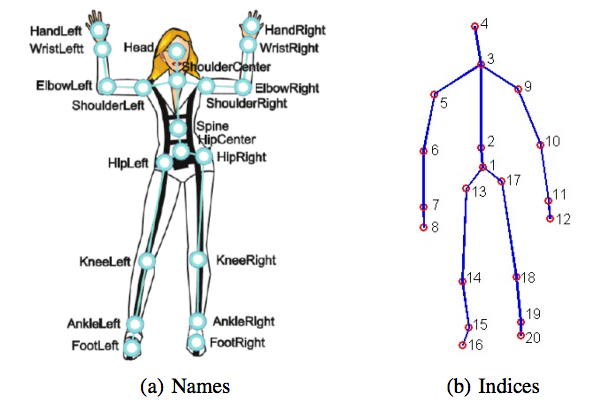
\includegraphics[width=0.5\textwidth]{skeleton_joint_names_indicies}
	\caption{Skeleton joint names and indices from Kinect SDK}
	\label{fig:kinect_sdk}
\end{figure}

The angles between two adjacent body extremities were also computed and stored as ($\theta_1^t,...,\theta_5^t$). Once finished processing the all the frames, a histogram for each \emph{$\textbf{d}_\textbf{i}$} and $ \boldsymbol\theta_\textbf{\emph{i}}$, i=1,...,5 are computed using bins N and M respectively. Each histogram is normalized by the total number of frames T to account for the different number of frames in each instance. A one dimensional feature vector is then concatenated from all the normalized histograms for form a single dimension vector of length 5(N+M). This feature vector is transformed into LIBSVM format where the label is the activity number (e.g. a08, the label would be 08), the index must start at one and is incremented by one, and the value at an index starts at the beginning of the feature vector and iterates until the end. Each feature vector in LIBSVM represents one instance (file) per line in rad and rad.t.

\begin{figure}
	\centering
	\includegraphics[width=0.5\textwidth]{star}
	\caption{Illustration of human representation based on relative distance and angles of star skeleton}
	\label{fig:star}
\end{figure}

\subsection{HJPD}

The second skeleton representation implemented is the Histogram of Joint Position Differences (HJPD), referenced in Section 3.3 of reference \cite{hjpdPaper}. HJPD is similar to RAD except it uses all joints given and not just six total points. Joint position differences also ignores any pairwise angles. HJPD starts by taking each joint in each frame and calculating the joint displacement between a reference joint and all other joints. Given a joint location (x, y, z) and a reference joint location ($x_c, y_c, z_c$), the joint displacement is defined as:
\begin{equation}
(\Delta{x}, \Delta{y}, \Delta{z}) = (x, y, z) - (x_c, y_c, z_c)
\end{equation}
The reference joint can be some fixed joint or the centroid of the skeleton. For the default representation the center of hip joint is used but experimentation was performed with the reference joint being a fixed joint that was not the centroid of the human skeleton. Once all distances are computed using the equation above, a histogram is computed for the displacement along each dimension (e.g.$ \Delta{x}, \Delta{y}, \Delta{z}$). These three histograms are concatenated to create a final feature vector and converted to LIBSVM format.

\subsection{HOD}

Skeleton data can be represented through a relatively new approach called Histogram of Oriented Displacements. This method is described in Section 3 from a recently published paper by [Gowayyed \textit{et al., 2013}]. The approach of this method is to create a 3D trajectory of each joint by first creating three 2D joints on the \emph{xy, yz, xz} orthogonal cartesian planes. The 3D trajectory is the concatenation of the three 2D trajectories. A 2D trajectory is referred to as HOD in \cite{hodPaper}. These 2D trajectories are described using a histogram with bins filled with the direction between two consecutive points. All 2D plane points are gathered together such that $all2DXY_i = \{ pXY_i^t \}$, t = 1,...,T and i = 1,...,20. The same is done for the \emph{yz} and \emph{xz} planes. Next a histogram of N bins is created for each $all2DXY_i, all2DYZ_i, all2DXZ_i, i = 1,...,20$ using the distance and angle calculated between $P_t$ and $P_{t+1}$ points. The angle is used to determine which bin the distance is placed in using:
\begin{equation}
histogram\_bin = \frac{angle * histogram\_length}{360}
\end{equation}

A key distinction for this implementation is that the bin is not incremented by one, instead the bin is incremented by the distance.

\begin{figure}
	\centering
	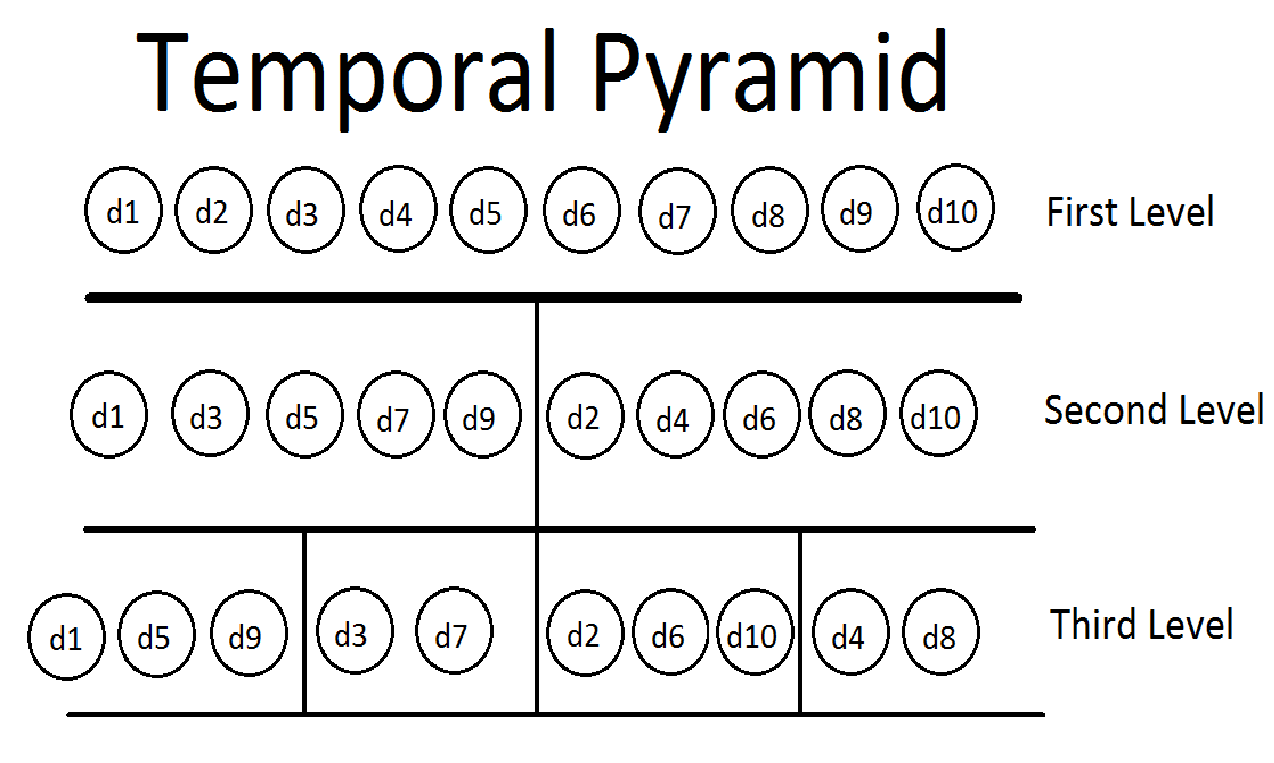
\includegraphics[width=0.5\textwidth]{temporal_pyramid2}
	\caption{A simple figure describing how the temporal pyramid splits the data.}
	\label{fig:hodPyramid}
\end{figure}

To account for missing temporal information, a temporal pyramid approach is implemented. At the first level of the pyramid, all trajectory information is used. At the next level, the trajectory information is divided in half and creates two histograms.  At any subsequent level, the trajectory is divided in half again. A three level pyramid would contain seven histograms, one for the first level, two for the second level, and four for the third level. These histograms will have their respective bins summed to form a final descriptor. For the implementation of the project, the trajectory information is not a clear split in half as described in \cite{hodPaper}. When the first level is divided, odd trajectories are used for the second level histograms (see figure \ref{fig:hodPyramid}). Once each \emph{xy, yz, xz} trajectory histograms are created, they are normalized by summing up the total distances from each bin and dividing individual bins by that total. Once the histograms are normalized, they are concatenated to produce the final 3D trajectory for a single point. After each point's 3D trajectory is computed, all 3D trajectories are concatenated and converted to LIBSVM format.

\section{Experiments}

Due to the high number of configurable parameters for RAD and number of joints to use for HJPD, majority of experiments were spent delving into making RAD and HJPD perform more accurately. The RAD program can accept many configuration options, which include the lower and upper bound and bin sizes for the histograms. Both distance and angle histograms were modified to test the effects the lower/upper bounds and bin sizes had on the performance. HJPD has four different tunable parameters: histogram lower bound, histogram upper bound, histogram bins, and the reference joint. The HOD program has fixed upper and lower bounds for the histograms so the only parameter to modify is the number of bins.

Starting with RAD, some default parameters for the lower and upper bounds of the histograms for angles and distances were chosen from the lowest and highest values seen while developing the program. For the distance histograms, a lower bound of 0.0 and upper bound of 2.2 were chosen. For the angle histograms, a lower bound of 0.0 and upper bound of 3.2 were chosen. As for the bins for each, sizes of 50 for distance and 20 angle were chosen at random. The default joints used were head, center of hip, both hands,  and both feet. All RAD experiments used the options provided by the program and any options not used are based on the default values mentioned above. Many experiments were conducted using these customizable parameters. The star skeleton was tested by using a combination of hands/feet, hands/ankles, wrists/feet, and wrists/ankles. Other experiments for RAD included modifying only the lower bound with the default upper bound and upper bound with the default lower bound at a constant rate of 0.05 up to half the range. For example the lower bound would be incremented by 0.05 until the value reached 1.6 (For distance u = 3.2, l = 0.0 (upper - lower) / 2) for the distance histograms. The same concept applies for the upper bound, except it is decremented by 0.05 until reaching 1.6. Bin size was separately modified for distance histograms ranging from 5 to 50 bins in increments of 5. These experiments were also conducted in the same manner for angle histograms. Other experiments included modifying both lower and upper bounds at the same constant rate of 0.05 with the end condition at one-fourth (0.00 to 0.8 lower, 3.2 to 2.4 upper) of the range instead of one-half the range. This was applied to both distance and angle in two separate tests. The last experiment for RAD combined the method of lower and upper bound modification along with changing the bin size for a small exhaustive approach.

For HJPD experiments, similar tests were used such as lower bound only, upper bound only, bin size modification, lower/upper modification at constant rate, and a combination of lower/upper modification with bin modification for another exhaustive approach. As with RAD, experiments that did not use options used the default values in the program as noted in the next few sentences. The default parameters for HJPD were chosen the same way RAD parameters were chosen, based on the lowest and highest values seen while development. The default lower and upper bound parameters were chosen to be -1.1 and 1.3 respectively. The default number of bins was randomly chosen to be 20. Reference joint 1, or center of hip was chosen as this is usually the most stable point on the body. All experiments used the same constraints (0.05 rate for bounds, increments of 5 for bins). The bounds for the lower tests ranged from -1.1 to 0.1 and upper tests ranged from 1.3 to 0.1. For the lower/upper and lower/upper/bin combinations, lower bounds were -1.1 to -0.5 and upper bounds were 1.3 to 0.7. One last test used this lower/upper/bin approach on all possible reference joints as well. 

HOD experiments were the easiest to conduct as this dealt with experimenting with the bin size, from 4 bins to 16 bins incrementing one at a time. The defaults for HOD are a lower bound of 0, upper bound of 360, and 6 bins. Other experiments were conducted in changing the number levels of the temporal pyramid to two- and one-level pyramids. This was done manually through the code as there was not an option made available to change this parameter.

\section{Results}

From the base implementations of each skeleton-based representation, accuracy rates of 54\%, 77\%, and 79\% for RAD, HJPD, and HOD respectively. For RAD results, the star skeleton joints were changed to see the effect wrists/ankle pairs compared to hands/feet pairs. From the tests, hands/feet, wrists/feet, and hands/ankles all had the same accuracy of 54\%. However, there was a 2\% increase in accuracy when using wrists/ankles as part of the star skeleton. Changes in distance histogram parameters had shown small increases in accuracy of 12\% increases with a lower value of 0.45 and upper value of 1.95. Out of the range of 5-50 bins, the bin size that offered the greatest increase in accuracy were 10 to 15 bin sizes. Changes in angle histogram parameters had increased accuracy about 6-10\% with a lower bound of 0.1 and upper bound of 2.15. The highest yield bin sizes were 40-45 bins. Using this new information, RAD was run using distance lower/upper/bin size 0.45 / 1.95 / 10 and angle lower/upper/bin size 0.1 / 2.15 / 40 along with wrist/ankle star skeleton joints. This produced an accuracy of 60\%, an overall increase of 6\%. From the experiments on RAD, for the data given, wrist and ankle joints perform slightly better than hand and feet joints for star skeleton representation.

\begin{table}[t]
\caption{HJPD: Reference Joint accuracy above 80\%}
\centering
\begin{tabular}{c c c c c c c}
\hline\hline
 & 81\% & 83\% & 85\% & 87\% & 89\% & Total \\ [0.5ex]
\hline
C. Hip & 19 & 13 & 4 & 4 & - & 40 \\
Spine & 6 & 4 & 1 & - & 1 & 12 \\
C. Shldr & 3 & - & - & - & - & 3 \\
L. Elbow & - & 1 & 1 & - & - & 2 \\
L. Wrist & 2 & - & - & - & - & 2 \\
R. Shldr & - & 1 & - & - & - & 1 \\
R. Elbow & 8 & 8 & 7 & - & - & 23 \\
R. Hand & 1 & - & - & - & - & 1 \\
L. Hip & 13 & 5 & 3 & - & - & 21 \\
L. Knee & 1 & - & - & - & - & 1 \\
R. Hip & 4 & - & - & - & - & 4 \\
\hline\hline
Total & 57 & 32 & 16 &  4 & 1 & 110 \\
\hline
\end{tabular}
\label{table:hjpdResult}
\end{table}

HJPD had more interesting results. The first few experiments of lower only, upper only, and bin size modification yielded relatively small increases in accuracy, from 2-8\% increases. A lower/upper/bin modification produced a few resulting parameters that increased accuracy up to 87\%. Some combinations of lower/upper/bin that boosted accuracy to 87\% were -1 / 1.2 / 15, -0.9 / 1.1 / 10, -0.85 / 1.05 / 10, and -0.5 / 0.7 / 10. Upon testing each joint with the lower/upper/bin modification, unusually reference joints showed up that produced accuracy ratings of 81\% and higher. If you take a look at table \ref{table:hjpdResult}, you can see that the hip center is the most stable joint for high accuracy. Though if you notice that right elbow and left hip also produce many high accuracy results. Both right elbow and left hip account for roughly 40\% of the total number of accuracies higher than 80\%. Other unusual joints that appear are shoulder center, left elbow, left wrist, right shoulder, right hand, left knee, and right hip. These results could be explained by how the data was recorded according to the write up. Most activities recorded were from a sitting position. This could attribute to the high percentage of right elbow and left hip accuracies. From reviewing the images in the project write-up, many positions have very stable right elbow positions as well as left hip positions. This could attribute to the high percentage of plausible right elbow/left hip reference joints producing high recognition accuracies. Even though the center hip joint produces a very stable amount of high accuracy, the spine was able to provide an accuracy as high as 89\%. From this data, HJPD was rerun with a lower bound of -0.55, upper bound of 0.75, 10 bins and the reference joint being the spine. The resulting accuracy was 89\%.

\begin{table}[h]
\caption{HJPD: Confusion Matrix 89\% Accuracy}
\centering
\begin{tabular}{c c c c c c c}
\hline\hline
 & 8 & 10 & 12 & 13 & 15 & 16 \\ [0.5ex]
\hline
8 & 7 & 1 & 0 & 0 & 0 & 0 \\
10 & 0 & 8 & 0 & 0 & 0 & 0 \\
12 & 0 & 0 & 8 & 0 & 0 & 0 \\
13 & 0 & 1 & 0 & 7 & 0 & 0 \\
15 & 0 & 1 & 0 & 0 & 5 & 2 \\
16 & 0 & 0 & 0 & 0 & 0 & 8 \\
\hline
\end{tabular}
\label{table:hjpdConfusion}
\end{table}

\begin{table}[h]
\caption{HOD: Confusion Matrix 91\% Accuracy}
\centering
\begin{tabular}{c c c c c c c}
\hline\hline
 & 8 & 10 & 12 & 13 & 15 & 16 \\ [0.5ex]
\hline
8 & 8 & 0 & 0 & 0 & 0 & 0 \\
10 & 1 & 7 & 0 & 0 & 0 & 0 \\
12 & 0 & 0 & 8 & 0 & 0 & 0 \\
13 & 0 & 0 & 1 & 7 & 0 & 0 \\
15 & 0 & 1 & 0 & 0 & 6 & 1 \\
16 & 0 & 0 & 0 & 0 & 0 & 8 \\
\hline
\end{tabular}
\label{table:hodConfusion}
\end{table}

The HOD implementation is a great skeleton-based representation as the lower accuracy was 72\% for bin sizes of 8 and 9. Bin sizes with the best accuracies were 10, 11, and 15 at 91\% accuracy. Compared to RAD and HJPD, HOD is the best of the three skeleton-based representation due to the fact that it can have at lease one customizable parameter and still perform with 90+\% accuracy. There was little work for a high accuracy from HOD. When compared to RAD, which one could modify at least ten different parameters, RAD required many experiments for a small increase in accuracy up to only 60\%. HJPD faired much better than RAD and almost hit a 90\% accuracy after tuning only four different parameters.

Another interest was to test loose and fine grid search to find a better C,gamma pair for better accuracy. Using a C$\pm$2 and gamma$\pm$2 for a fine grid search on the best accuracy runs for RAD, HJPD, and HOD, there were better C,gamma pairs found using grid with higher cross-validation rates. When using these finer tuned C's and gammas, they resulted in lower accuracies. Only HOD fine grid search did not change the accuracy when using the finer C,gamma pair. See the appendix for loose and fine grid search graphs for RAD, HJPD, and HOD. Using the fine grid search for RAD, it turns out that accuracy fell 4\%. When using the C,gamma pair from the finer grid search on HJPD, this resulted in an accuracy loss of 10\%. Compared to both RAD and HJPD fine grid searches, the fine grid C,gamma pair did not affect HOD, which resulted in a 91\% accuracy, same as the coarse C,gamma pair. As mentioned in \cite{guide}, their support vector guide, the fine grid search approach works well with datasets of thousands or more points. This could be the reason that a fine grid search gave C,gamma pairs that performed more poorly than a loose grid search. The data used in the project does not contain enough data points for fine grid search to improve accuracy of any of the three skeleton-based implementations.

\section{Discussion}

Determining which skeleton-based representation is more useful depends on the accuracy and ease of parameter tuning. According to both of those expectation, HOD represented skeleton base actions the most accurately and with little hassle when tuning. Although this project implementation of HOD reached 91\% accuracy, [Gowayyed \textit{et al.}] was able to achieve an accuracy rating of 97.27\% with 4- and 8-bins with a three level temporal pyramid. The difference in accuracy from the project implementation and \cite{hodPaper} could be that the project constrained all C-SVMs use the RBF kernel as the learner while [Gowayyed \textit{et al.}] used linear kernels.

As mentioned earlier, HJPD can produce some unusually high accuracies using joints such as right elbow and left hip as reference joints. This result is significant due to the positions depicted from the dataset images in the project write-up. Roughly 14 of the 16 images features the subject in a sitting position. This could lead to stability in the right elbow and left hip joint 3D positions. This would ultimately cause HOD to classify these images with unintuitive high accuracy rates using an unorthodox reference joint.

% We recommend abbrvnat bibliography style.

\bibliographystyle{abbrvnat}

% The bibliography should be embedded for final submission.

\begin{thebibliography}
\softraggedright

\bibitem[Hsu et~al.(2010)Hsu, Chih-Wei]{guide}
C. Hsu, C. Chang, and C. Lin, "A Practical Guide to Support Vector Classification", Department of Computer Science, National Taiwan University, Taipei 106, Taiwan, April 15, 2010.

\bibitem[Rahmani et~al.(2014)Rahmani, Hossein]{hjpdPaper}
H. Rahmani, A. Mahmood, A. Mian, and D. Huynh, "Real time action recognition using histograms of depth gradients and random decision forests," in \textit{IEEE Winter Conference on Applications of Computer Vision}, 2014.

\bibitem[Gowayyed et~al.(2013)Gowayyed, Mohammad]{hodPaper}
M. Gowayyed, M. Torki, M. Hussein, and M. El-Saban, "Histogram of oriented displacements (HOD): Describing trajectories of human joints for action recognition," in \textit{International Joint Conference on Artificial Intelligence}, 2013.

\bibitem[Zhang(2014)Zhang, Hao]{projectWriteup}
H. Zhang, "CSCI498B/598B Human-Centered Robotics Project 2: Skeleton-Based Representations for Human Behavior Understanding," 2014.

\end{thebibliography}

\appendix
\section{Appendix: Grid Search Graphs}

\begin{figure}[h]
	\centering
	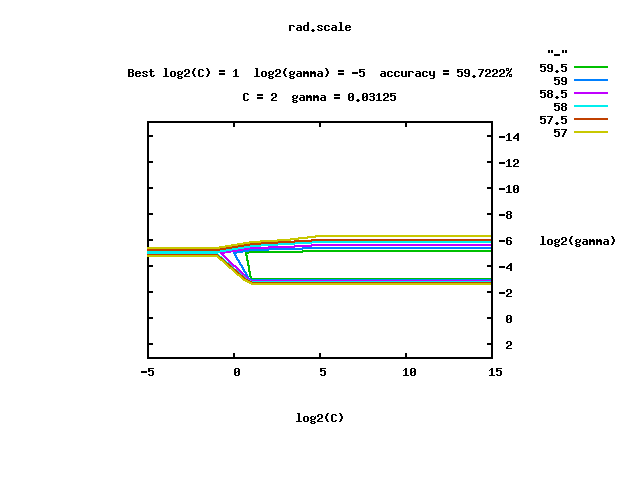
\includegraphics[width=0.55\textwidth]{coarseGridRad}
	\caption{RAD: Loose Grid search on C = $2^-5,...,2^15$ and $\gamma=2^-15,...,2^3$.}
	\label{fig:looseRad}
\end{figure}
\begin{figure}[p]
	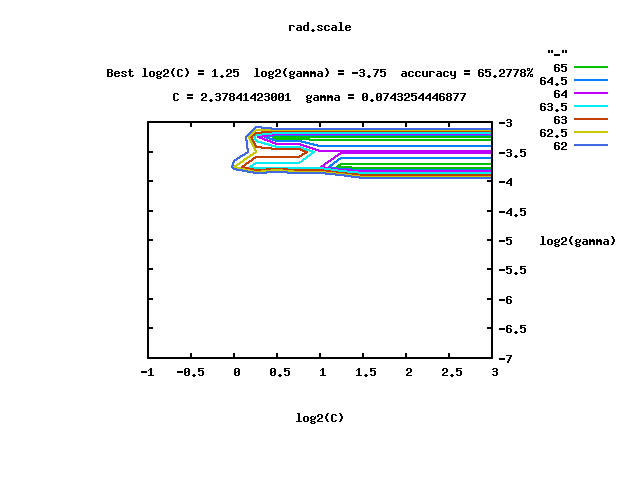
\includegraphics[width=0.55\textwidth]{fineGridRad}
	\caption{RAD: Fine Grid search on C = $2^-1,...,2^3$ and $\gamma=2^-7,...,2^3$.}
	\label{fig:fineRad}
	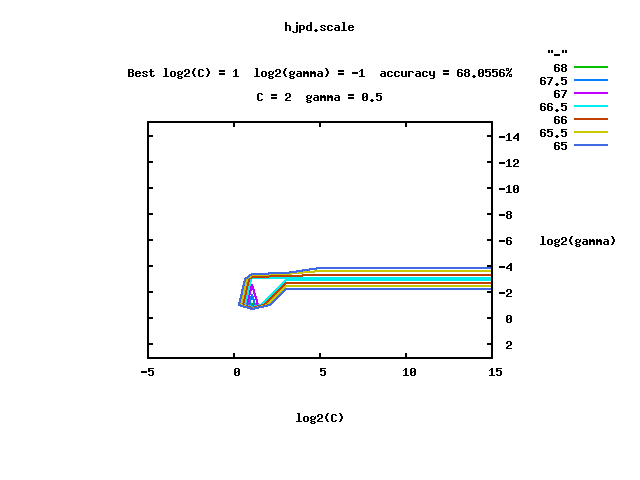
\includegraphics[width=0.55\textwidth]{coarseGridHjpd}
	\caption{HJPD: Loose Grid search on C = $2^-5,...,2^15$ and $\gamma=2^-15,...,2^3$.}
	\label{fig:looseHjpd}
	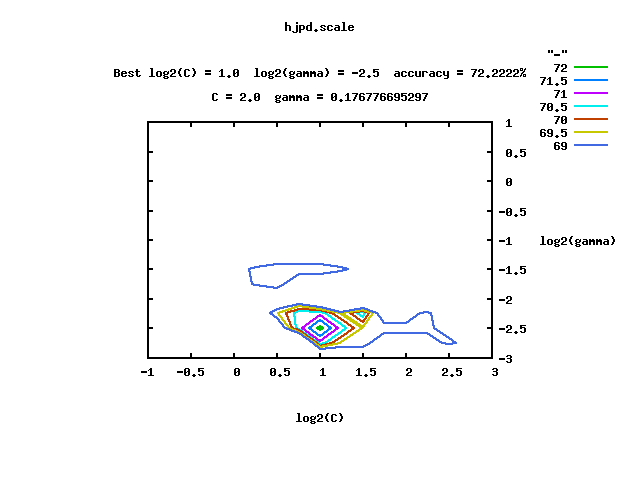
\includegraphics[width=0.5\textwidth]{fineGridHjpd}
	\caption{HJPD: Fine Grid search on C = $2^-1,...,2^3$ and $\gamma=2^-3,...,2^1$.}
	\label{fig:fineHjpd}
\end{figure}
\begin{figure}[p]
	\centering
	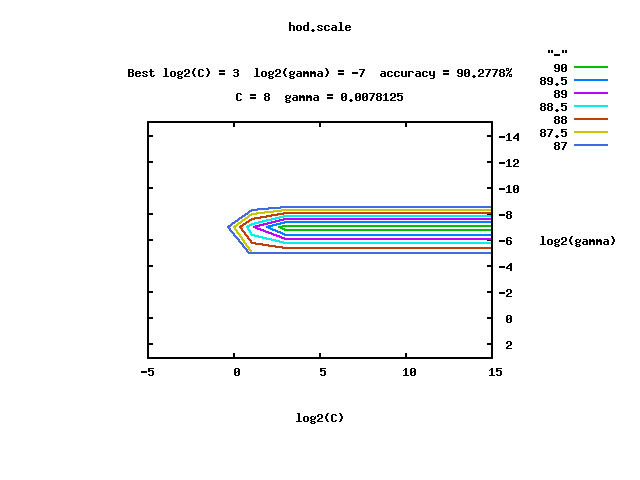
\includegraphics[width=0.55\textwidth]{coarseGridHod}
	\caption{HOD: Loose Grid search on C = $2^-5,...,2^15$ and $\gamma=2^-15,...,2^3$.}
	\label{fig:looseHod}
	\centering
	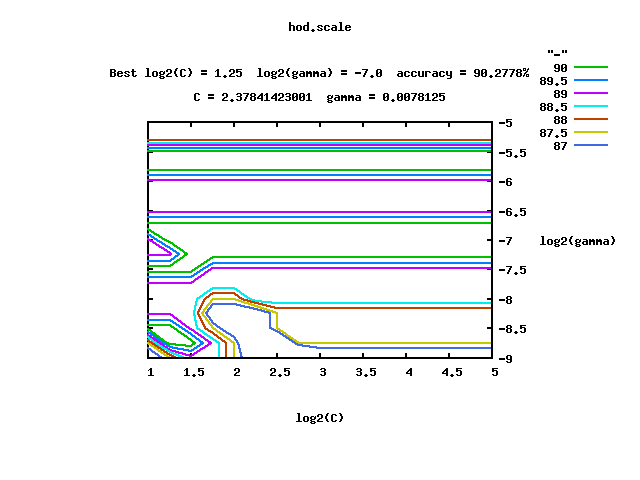
\includegraphics[width=0.55\textwidth]{fineGridHod}
	\caption{HOD: Fine Grid search on C = $2^1,...,2^5$ and $\gamma=2^-9,...,2^-5$.}
	\label{fig:fineHod}
\end{figure}

\end{document}
